% IEEE report -- Heart Disease Risk Modelling via Bayesian Networks and Feed-Forward Neural Networks
% All numbers in the text are macros from tables/numbers.tex, generated from results/metrics/*
% by `python -m src.evaluation.make_report_assets`. Build: see reports/README.md.
\documentclass[conference]{IEEEtran}
\usepackage{amsmath,amssymb}
\usepackage{graphicx}
\usepackage{booktabs}
\usepackage{url}
\usepackage{cite}
% Generated by src/evaluation/make_report_assets.py -- do not edit.
\newcommand{\BNHiObs}{0.946}
\newcommand{\BNHiPred}{0.979}
\newcommand{\BNHiShare}{30}
\newcommand{\BNLoObs}{0.092}
\newcommand{\BNLoPred}{0.025}
\newcommand{\BNLoShare}{37}
\newcommand{\BNYoudenMax}{0.78}
\newcommand{\BNYoudenMean}{0.55}
\newcommand{\BNYoudenMin}{0.21}
\newcommand{\BNalphaTop}{25}
\newcommand{\BNbrierCIHi}{0.157}
\newcommand{\BNbrierCILo}{0.099}
\newcommand{\BNbrierEst}{0.127}
\newcommand{\BNbrierMean}{0.127}
\newcommand{\BNbrierSD}{0.030}
\newcommand{\BNbrierYMean}{0.127}
\newcommand{\BNbrierYSD}{0.030}
\newcommand{\BNcalintPMean}{-0.06}
\newcommand{\BNcalintPSD}{0.03}
\newcommand{\BNcalslopePMean}{0.62}
\newcommand{\BNcalslopePSD}{0.01}
\newcommand{\BNeceMean}{0.122}
\newcommand{\BNecePMean}{0.082}
\newcommand{\BNecePSD}{0.003}
\newcommand{\BNeceSD}{0.029}
\newcommand{\BNeceYMean}{0.122}
\newcommand{\BNeceYSD}{0.029}
\newcommand{\BNfnP}{29.6}
\newcommand{\BNfoneMean}{0.799}
\newcommand{\BNfoneSD}{0.054}
\newcommand{\BNfoneYMean}{0.787}
\newcommand{\BNfoneYSD}{0.054}
\newcommand{\BNfpP}{25.0}
\newcommand{\BNloglossCIHi}{0.519}
\newcommand{\BNloglossCILo}{0.325}
\newcommand{\BNloglossEst}{0.416}
\newcommand{\BNloglossMean}{0.417}
\newcommand{\BNloglossSD}{0.106}
\newcommand{\BNloglossYMean}{0.417}
\newcommand{\BNloglossYSD}{0.106}
\newcommand{\BNpraucCIHi}{0.939}
\newcommand{\BNpraucCILo}{0.860}
\newcommand{\BNpraucEst}{0.905}
\newcommand{\BNpraucMean}{0.911}
\newcommand{\BNpraucSD}{0.037}
\newcommand{\BNpraucYMean}{0.911}
\newcommand{\BNpraucYSD}{0.037}
\newcommand{\BNprecMean}{0.818}
\newcommand{\BNprecSD}{0.066}
\newcommand{\BNprecYMean}{0.825}
\newcommand{\BNprecYSD}{0.082}
\newcommand{\BNrocaucCIHi}{0.939}
\newcommand{\BNrocaucCILo}{0.873}
\newcommand{\BNrocaucEst}{0.909}
\newcommand{\BNrocaucMean}{0.912}
\newcommand{\BNrocaucSD}{0.036}
\newcommand{\BNrocaucYMean}{0.912}
\newcommand{\BNrocaucYSD}{0.036}
\newcommand{\BNsensCIHi}{0.849}
\newcommand{\BNsensCILo}{0.719}
\newcommand{\BNsensEst}{0.787}
\newcommand{\BNsensMean}{0.787}
\newcommand{\BNsensSD}{0.083}
\newcommand{\BNsensYMean}{0.767}
\newcommand{\BNsensYSD}{0.109}
\newcommand{\BNspecCIHi}{0.895}
\newcommand{\BNspecCILo}{0.794}
\newcommand{\BNspecEst}{0.848}
\newcommand{\BNspecMean}{0.848}
\newcommand{\BNspecSD}{0.065}
\newcommand{\BNspecYMean}{0.851}
\newcommand{\BNspecYSD}{0.090}
\newcommand{\BNtnP}{139.0}
\newcommand{\BNtpP}{109.4}
\newcommand{\DOhigh}{14}
\newcommand{\DOlow}{11}
\newcommand{\DiffBNMLPbrierEst}{+0.005}
\newcommand{\DiffBNMLPbrierHi}{+0.019}
\newcommand{\DiffBNMLPbrierLo}{-0.008}
\newcommand{\DiffBNMLPloglossEst}{+0.025}
\newcommand{\DiffBNMLPloglossHi}{+0.080}
\newcommand{\DiffBNMLPloglossLo}{-0.027}
\newcommand{\DiffBNMLPpraucEst}{+0.010}
\newcommand{\DiffBNMLPpraucHi}{+0.032}
\newcommand{\DiffBNMLPpraucLo}{-0.011}
\newcommand{\DiffBNMLProcaucEst}{+0.005}
\newcommand{\DiffBNMLProcaucHi}{+0.021}
\newcommand{\DiffBNMLProcaucLo}{-0.012}
\newcommand{\DiffBNMLPsensEst}{-0.016}
\newcommand{\DiffBNMLPsensHi}{+0.020}
\newcommand{\DiffBNMLPsensLo}{-0.053}
\newcommand{\DiffBNMLPspecEst}{-0.017}
\newcommand{\DiffBNMLPspecHi}{+0.022}
\newcommand{\DiffBNMLPspecLo}{-0.058}
\newcommand{\DiffBNNBbrierEst}{-0.008}
\newcommand{\DiffBNNBbrierHi}{+0.002}
\newcommand{\DiffBNNBbrierLo}{-0.017}
\newcommand{\DiffBNNBloglossEst}{-0.048}
\newcommand{\DiffBNNBloglossHi}{-0.018}
\newcommand{\DiffBNNBloglossLo}{-0.081}
\newcommand{\DiffBNNBpraucEst}{+0.005}
\newcommand{\DiffBNNBpraucHi}{+0.015}
\newcommand{\DiffBNNBpraucLo}{-0.004}
\newcommand{\DiffBNNBrocaucEst}{+0.004}
\newcommand{\DiffBNNBrocaucHi}{+0.013}
\newcommand{\DiffBNNBrocaucLo}{-0.004}
\newcommand{\DiffBNNBsensEst}{-0.016}
\newcommand{\DiffBNNBsensHi}{+0.009}
\newcommand{\DiffBNNBsensLo}{-0.043}
\newcommand{\DiffBNNBspecEst}{-0.002}
\newcommand{\DiffBNNBspecHi}{+0.023}
\newcommand{\DiffBNNBspecLo}{-0.029}
\newcommand{\DiffNBMLPbrierEst}{+0.013}
\newcommand{\DiffNBMLPbrierHi}{+0.029}
\newcommand{\DiffNBMLPbrierLo}{-0.002}
\newcommand{\DiffNBMLPloglossEst}{+0.073}
\newcommand{\DiffNBMLPloglossHi}{+0.145}
\newcommand{\DiffNBMLPloglossLo}{+0.007}
\newcommand{\DiffNBMLPpraucEst}{+0.005}
\newcommand{\DiffNBMLPpraucHi}{+0.028}
\newcommand{\DiffNBMLPpraucLo}{-0.016}
\newcommand{\DiffNBMLProcaucEst}{+0.001}
\newcommand{\DiffNBMLProcaucHi}{+0.016}
\newcommand{\DiffNBMLProcaucLo}{-0.014}
\newcommand{\DiffNBMLPsensEst}{+0.000}
\newcommand{\DiffNBMLPsensHi}{+0.032}
\newcommand{\DiffNBMLPsensLo}{-0.033}
\newcommand{\DiffNBMLPspecEst}{-0.015}
\newcommand{\DiffNBMLPspecHi}{+0.023}
\newcommand{\DiffNBMLPspecLo}{-0.055}
\newcommand{\MLPHiObs}{0.979}
\newcommand{\MLPHiPred}{0.937}
\newcommand{\MLPHiShare}{9}
\newcommand{\MLPLoObs}{0.037}
\newcommand{\MLPLoPred}{0.055}
\newcommand{\MLPLoShare}{23}
\newcommand{\MLPYoudenMax}{0.71}
\newcommand{\MLPYoudenMean}{0.55}
\newcommand{\MLPYoudenMin}{0.35}
\newcommand{\MLPbrierCIHi}{0.144}
\newcommand{\MLPbrierCILo}{0.099}
\newcommand{\MLPbrierEst}{0.121}
\newcommand{\MLPbrierMean}{0.121}
\newcommand{\MLPbrierSD}{0.025}
\newcommand{\MLPbrierYMean}{0.121}
\newcommand{\MLPbrierYSD}{0.025}
\newcommand{\MLPcalintPMean}{0.09}
\newcommand{\MLPcalintPSD}{0.10}
\newcommand{\MLPcalslopePMean}{1.10}
\newcommand{\MLPcalslopePSD}{0.05}
\newcommand{\MLPeceMean}{0.113}
\newcommand{\MLPecePMean}{0.059}
\newcommand{\MLPecePSD}{0.009}
\newcommand{\MLPeceSD}{0.033}
\newcommand{\MLPeceYMean}{0.113}
\newcommand{\MLPeceYSD}{0.033}
\newcommand{\MLPfnP}{27.4}
\newcommand{\MLPfoneMean}{0.817}
\newcommand{\MLPfoneSD}{0.059}
\newcommand{\MLPfoneYMean}{0.816}
\newcommand{\MLPfoneYSD}{0.057}
\newcommand{\MLPfpP}{22.2}
\newcommand{\MLPloglossCIHi}{0.452}
\newcommand{\MLPloglossCILo}{0.332}
\newcommand{\MLPloglossEst}{0.391}
\newcommand{\MLPloglossMean}{0.391}
\newcommand{\MLPloglossSD}{0.064}
\newcommand{\MLPloglossYMean}{0.391}
\newcommand{\MLPloglossYSD}{0.064}
\newcommand{\MLPpraucCIHi}{0.933}
\newcommand{\MLPpraucCILo}{0.851}
\newcommand{\MLPpraucEst}{0.895}
\newcommand{\MLPpraucMean}{0.905}
\newcommand{\MLPpraucSD}{0.040}
\newcommand{\MLPpraucYMean}{0.905}
\newcommand{\MLPpraucYSD}{0.040}
\newcommand{\MLPprecMean}{0.837}
\newcommand{\MLPprecSD}{0.067}
\newcommand{\MLPprecYMean}{0.863}
\newcommand{\MLPprecYSD}{0.070}
\newcommand{\MLProcaucCIHi}{0.936}
\newcommand{\MLProcaucCILo}{0.868}
\newcommand{\MLProcaucEst}{0.903}
\newcommand{\MLProcaucMean}{0.907}
\newcommand{\MLProcaucSD}{0.037}
\newcommand{\MLProcaucYMean}{0.907}
\newcommand{\MLProcaucYSD}{0.037}
\newcommand{\MLPsensCIHi}{0.862}
\newcommand{\MLPsensCILo}{0.737}
\newcommand{\MLPsensEst}{0.803}
\newcommand{\MLPsensMean}{0.803}
\newcommand{\MLPsensSD}{0.080}
\newcommand{\MLPsensYMean}{0.780}
\newcommand{\MLPsensYSD}{0.083}
\newcommand{\MLPspecCIHi}{0.908}
\newcommand{\MLPspecCILo}{0.819}
\newcommand{\MLPspecEst}{0.865}
\newcommand{\MLPspecMean}{0.865}
\newcommand{\MLPspecSD}{0.059}
\newcommand{\MLPspecYMean}{0.890}
\newcommand{\MLPspecYSD}{0.064}
\newcommand{\MLPtnP}{141.8}
\newcommand{\MLPtpP}{111.6}
\newcommand{\NBHiObs}{0.924}
\newcommand{\NBHiPred}{0.983}
\newcommand{\NBHiShare}{31}
\newcommand{\NBLoObs}{0.110}
\newcommand{\NBLoPred}{0.020}
\newcommand{\NBLoShare}{40}
\newcommand{\NBYoudenMax}{0.80}
\newcommand{\NBYoudenMean}{0.52}
\newcommand{\NBYoudenMin}{0.31}
\newcommand{\NBalphaTop}{25}
\newcommand{\NBbrierCIHi}{0.166}
\newcommand{\NBbrierCILo}{0.105}
\newcommand{\NBbrierEst}{0.134}
\newcommand{\NBbrierMean}{0.134}
\newcommand{\NBbrierSD}{0.031}
\newcommand{\NBbrierYMean}{0.134}
\newcommand{\NBbrierYSD}{0.031}
\newcommand{\NBcalintPMean}{-0.05}
\newcommand{\NBcalintPSD}{0.02}
\newcommand{\NBcalslopePMean}{0.51}
\newcommand{\NBcalslopePSD}{0.00}
\newcommand{\NBeceMean}{0.139}
\newcommand{\NBecePMean}{0.101}
\newcommand{\NBecePSD}{0.010}
\newcommand{\NBeceSD}{0.027}
\newcommand{\NBeceYMean}{0.139}
\newcommand{\NBeceYSD}{0.027}
\newcommand{\NBfnP}{27.4}
\newcommand{\NBfoneMean}{0.810}
\newcommand{\NBfoneSD}{0.056}
\newcommand{\NBfoneYMean}{0.800}
\newcommand{\NBfoneYSD}{0.058}
\newcommand{\NBfpP}{24.6}
\newcommand{\NBloglossCIHi}{0.589}
\newcommand{\NBloglossCILo}{0.354}
\newcommand{\NBloglossEst}{0.465}
\newcommand{\NBloglossMean}{0.465}
\newcommand{\NBloglossSD}{0.109}
\newcommand{\NBloglossYMean}{0.465}
\newcommand{\NBloglossYSD}{0.109}
\newcommand{\NBpraucCIHi}{0.936}
\newcommand{\NBpraucCILo}{0.853}
\newcommand{\NBpraucEst}{0.900}
\newcommand{\NBpraucMean}{0.907}
\newcommand{\NBpraucSD}{0.035}
\newcommand{\NBpraucYMean}{0.907}
\newcommand{\NBpraucYSD}{0.035}
\newcommand{\NBprecMean}{0.825}
\newcommand{\NBprecSD}{0.072}
\newcommand{\NBprecYMean}{0.824}
\newcommand{\NBprecYSD}{0.078}
\newcommand{\NBrocaucCIHi}{0.935}
\newcommand{\NBrocaucCILo}{0.869}
\newcommand{\NBrocaucEst}{0.904}
\newcommand{\NBrocaucMean}{0.907}
\newcommand{\NBrocaucSD}{0.033}
\newcommand{\NBrocaucYMean}{0.907}
\newcommand{\NBrocaucYSD}{0.033}
\newcommand{\NBsensCIHi}{0.863}
\newcommand{\NBsensCILo}{0.736}
\newcommand{\NBsensEst}{0.803}
\newcommand{\NBsensMean}{0.803}
\newcommand{\NBsensSD}{0.090}
\newcommand{\NBsensYMean}{0.786}
\newcommand{\NBsensYSD}{0.087}
\newcommand{\NBspecCIHi}{0.897}
\newcommand{\NBspecCILo}{0.795}
\newcommand{\NBspecEst}{0.850}
\newcommand{\NBspecMean}{0.850}
\newcommand{\NBspecSD}{0.068}
\newcommand{\NBspecYMean}{0.851}
\newcommand{\NBspecYSD}{0.075}
\newcommand{\NBtnP}{139.4}
\newcommand{\NBtpP}{111.6}
\newcommand{\WDhigh}{16}
\newcommand{\WDlow}{9}
\newcommand{\foldHash}{3ece83bae3e0a960}
\newcommand{\missCa}{4}
\newcommand{\missThal}{2}
\newcommand{\nBoot}{2000}
\newcommand{\nMissRows}{6}
\newcommand{\nNeg}{164}
\newcommand{\nOuter}{25}
\newcommand{\nParamsMLP}{481}
\newcommand{\nPatients}{303}
\newcommand{\nPos}{139}
\newcommand{\numFour}{13}
\newcommand{\numOne}{55}
\newcommand{\numThree}{35}
\newcommand{\numTwo}{36}
\newcommand{\numZero}{164}
\newcommand{\posPct}{45.9}
\newcommand{\seed}{42}

\graphicspath{{figures/}}

\begin{document}

\title{Heart Disease Risk Modelling via Bayesian Networks and Feed-Forward Neural Networks: A Small-Sample Comparison with Nested Cross-Validation}

\author{\IEEEauthorblockN{[Author names to be added by the team]}
\IEEEauthorblockA{[Institution, department, e-mail]}}

\maketitle

\begin{abstract}
We compare three probabilistic classifiers for angiographically defined heart disease on the Cleveland subset of the UCI Heart Disease data ($n=\nPatients$, $\nPos$ positive): a domain-informed Bayesian network, a Naive Bayes baseline and a small feed-forward neural network (MLP, \nParamsMLP\ parameters). All data-dependent preprocessing is fitted inside training folds, hyper-parameters are tuned by nested cross-validation, and all models are scored on identical $5\times5$ stratified outer folds. Discrimination is nearly identical: pooled out-of-fold ROC AUC is \BNrocaucEst\ [\BNrocaucCILo, \BNrocaucCIHi] for the Bayesian network, \NBrocaucEst\ [\NBrocaucCILo, \NBrocaucCIHi] for Naive Bayes and \MLProcaucEst\ [\MLProcaucCILo, \MLProcaucCIHi] for the MLP (95\% patient-level bootstrap intervals); no paired AUC difference is distinguishable from zero. Probability quality differs more: the MLP has the best Brier score (\MLPbrierEst) and calibration slope (\MLPcalslopePMean), whereas the Bayesian network (\BNcalslopePMean) and Naive Bayes (\NBcalslopePMean) are over-confident. With one centre, 303 patients and no external validation, these results are internal estimates for an academic comparison and do not demonstrate clinical validity.
\end{abstract}

\begin{IEEEkeywords}
Bayesian network, Naive Bayes, neural network, calibration, nested cross-validation, heart disease, small data
\end{IEEEkeywords}

%--------------------------------------------------------------------
\section{Introduction and Research Motivation}
Estimating the probability that a patient has coronary artery disease from routine and exercise-test findings is a classic problem in clinical prediction. For decision support a classifier should not only rank patients correctly but also output \emph{calibrated} probabilities \cite{steyerberg2010,vancalster2019}. Three model families offer different trade-offs. A Bayesian network (BN) encodes assumed dependencies explicitly and yields a posterior distribution by exact inference \cite{pearl1988,koller2009}. Naive Bayes is the simplest BN and a standard baseline despite its strong independence assumption \cite{domingos1997}. A neural network can learn arbitrary interactions but has many parameters relative to a dataset of a few hundred rows.

This work asks a narrow, testable question: \emph{on the Cleveland data, under a leakage-safe and identical evaluation protocol, do a domain-informed BN, Naive Bayes and a small MLP differ in discrimination and in probability calibration, and how large is the uncertainty about those differences?} The study is academic machine-learning research; it is not a diagnostic tool.

%--------------------------------------------------------------------
\section{Related Work and Literature Review}
The four databases in the archive (Cleveland, Hungarian, Swiss and Long Beach VA) are associated with the international evaluation of a probability algorithm for coronary disease diagnosis by Detrano \emph{et al.} \cite{detrano1989}, and are distributed through the UCI repository \cite{uciheart}. We use only the Cleveland file.

\emph{Bayesian classifiers.} Pearl \cite{pearl1988} and Koller and Friedman \cite{koller2009} give the theory of Bayesian networks and exact inference. Heckerman \emph{et al.} \cite{heckerman1995} show how prior domain knowledge and data can be combined when learning networks, which motivates fixing a structure from domain knowledge and estimating only the probability tables from data. Domingos and Pazzani \cite{domingos1997} show that Naive Bayes can be accurate for classification even when its independence assumption is violated, because classification depends only on the ranking of posteriors, not on their exact values; this implies that probability estimates, rather than rankings, are where violated independence should show.

\emph{Neural networks and tabular data.} Dropout \cite{srivastava2014}, weight decay and early stopping regularise networks, and Adam \cite{kingma2015} is a standard optimiser. On tabular data, neural networks are not consistently better than simpler alternatives \cite{shwartz2022,grinsztajn2022}, so a small network is not expected to win on 303 rows. Guo \emph{et al.} \cite{guo2017} report that modern deep networks tend to be over-confident; Niculescu-Mizil and Caruana \cite{niculescu2005} compare the calibration of several supervised learners. Our small, regularised MLP is a different regime from the large networks studied in \cite{guo2017}.

\emph{Evaluation.} Cross-validation used for both tuning and reporting gives optimistic estimates, which nested cross-validation avoids \cite{varma2006,cawley2010}. Information leaking from test data into preprocessing or model selection is a common cause of irreproducible results \cite{kapoor2023}. ROC curves \cite{fawcett2006,hanley1982} and precision--recall curves \cite{davis2006} summarise ranking; the Brier score \cite{brier1950} and calibration slope \cite{steyerberg2010,vancalster2019} summarise probability quality. Rudin \cite{rudin2019} cautions against treating post-hoc explanations of black-box models as faithful accounts of the underlying phenomenon. Reporting guidance for prediction models is given by TRIPOD \cite{collins2015}; this study does not claim full TRIPOD compliance.

\emph{Scope.} We did not perform a systematic survey of the many published studies on this dataset. Their accuracy figures are not compared here, because protocols (splits, preprocessing, tuning, threshold choice) differ and are often not reported in enough detail to make such comparisons reliable.

%--------------------------------------------------------------------
\section{Dataset Description and Exploratory Analysis}
\textbf{Source.} We use \texttt{processed.cleveland.data} from the UCI Heart Disease archive \cite{uciheart} (CC BY 4.0). The archive's own notice states that the unprocessed \texttt{cleveland.data} is corrupted and the processed file is the usable one. The file has no header; we assign the documented order \texttt{age, sex, cp, trestbps, chol, fbs, restecg, thalach, exang, oldpeak, slope, ca, thal, num}.

\textbf{Observed properties.} The file has $\nPatients$ rows and 14 columns, no duplicate rows, and no value outside the documented domains. Missing values (marked ``?'') occur only in \texttt{ca} ($\missCa$) and \texttt{thal} ($\missThal$), affecting $\nMissRows$ rows. The original diagnosis \texttt{num} has counts $\numZero/\numOne/\numTwo/\numThree/\numFour$ for levels $0$--$4$.

\textbf{Target.} We define $y=0$ if \texttt{num}$=0$ and $y=1$ if \texttt{num}$\in\{1,2,3,4\}$; any other value raises an error. This gives $\nNeg$ negative and $\nPos$ positive patients ($\posPct\%$ positive), so class imbalance is mild. The original five-level label is preserved but unused, and the binarisation discards severity information.

\textbf{Exploratory findings} (descriptive; no significance is claimed). Only one predictor pair has $|\rho_{\text{Spearman}}|\ge 0.5$ (\texttt{oldpeak}--\texttt{slope}, $0.595$), and no feature duplicates another. Several category levels are sparse (\texttt{restecg}$=1$: 4 rows; \texttt{thal}$=6$: 18; \texttt{ca}$=3$: 20). Asymptomatic chest pain (\texttt{cp}$=4$) has the highest positive rate ($0.729$), which probably reflects referral into angiography rather than a protective effect. There are no identifier or date columns and no predictor is derived from the target; however, \texttt{ca}, \texttt{thal}, \texttt{oldpeak}, \texttt{slope}, \texttt{exang} and \texttt{thalach} come from exercise testing, fluoroscopy and perfusion imaging, so the setting is a diagnostic work-up rather than first-contact triage. Fig.~\ref{fig:eda} shows the target distribution and predictor correlations.

\begin{figure}[t]
\centering
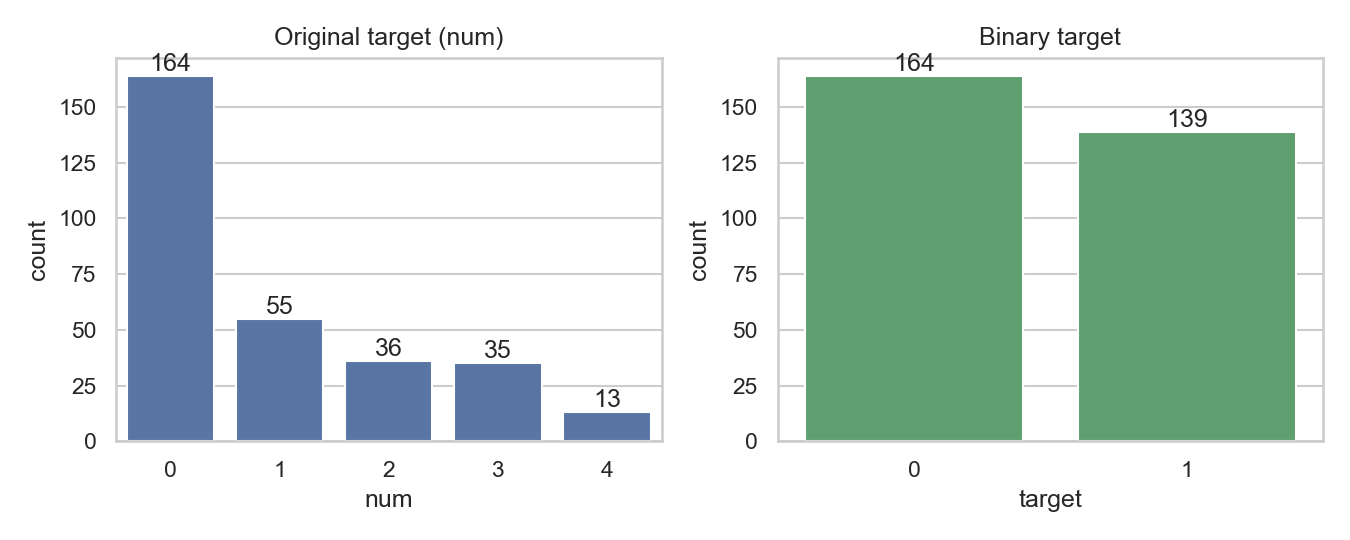
\includegraphics[width=\columnwidth]{eda_target_distribution.png}\\[2pt]
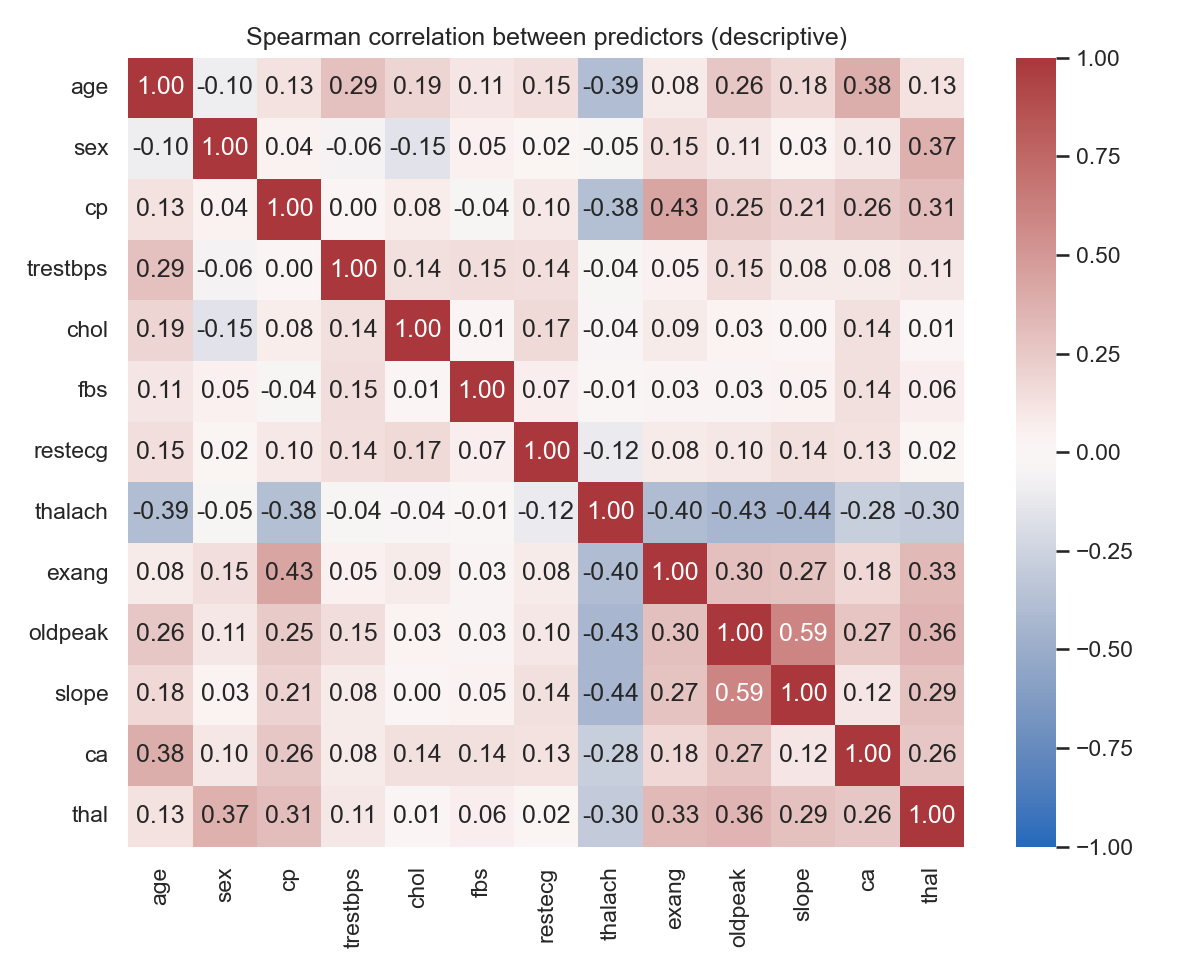
\includegraphics[width=0.92\columnwidth]{eda_correlation_heatmap.png}
\caption{Original and binary target distributions, and Spearman correlations between predictors.}
\label{fig:eda}
\end{figure}

\textbf{Correlation is not causation.} Associations in this sample can arise from confounding (e.g.\ age), selection into catheterisation, or reverse relationships. Nothing in the exploratory analysis or in the models below identifies causal effects.

%--------------------------------------------------------------------
\section{Feature Engineering and Preprocessing}
Features are grouped by type from the dataset documentation: \emph{continuous} (\texttt{age, trestbps, chol, thalach, oldpeak}), \emph{binary} (\texttt{sex, fbs, exang}), \emph{ordinal} (\texttt{ca}; \texttt{slope}: up $<$ flat $<$ down) and \emph{nominal} (\texttt{cp, restecg, thal}; numeric codes carry no order, e.g.\ \texttt{thal} $\in\{3,6,7\}$). Both pipelines begin with a guard that rejects the target columns, so the target cannot be used as a predictor.

\textbf{Missing values.} Missing \texttt{ca} and \texttt{thal} are imputed with the training-fold mode (median for continuous features, for which none are missing). With only $\nMissRows$ affected rows this is a simple choice; it ignores uncertainty about the missing value.

\textbf{MLP pipeline.} After imputation, continuous and ordinal features are standardised using training-fold means and variances, and nominal features are one-hot encoded with categories from the training fold (an unseen category maps to all zeros), giving 20 input columns.

\textbf{BN / Naive Bayes pipeline.} These models use conditional probability tables and need finite state spaces. Continuous features are cut into three train-fold quantile bins (tertiles; duplicate edges collapse when ties dominate, e.g.\ \texttt{oldpeak}), and all features are integer-coded from the training vocabulary. Missing or unseen values become the training mode. Tertiles keep each table small for $n=\nPatients$ and avoid assuming clinical cut-points.

\textbf{Leakage control.} Every quantity learned from data (imputation values, scaling statistics, categories, bin edges, vocabularies) is learned in \texttt{fit} on the training data of the current fold, and the whole pipeline is re-fitted in each inner and outer fold. The preprocessing design was fixed from the data documentation and the audit, before any model was evaluated.

%--------------------------------------------------------------------
\section{Theoretical Methodology}
\label{sec:theory}
\textbf{Bayes' rule and conditional independence.} For a class $Y\in\{0,1\}$ and predictors $\mathbf X=(X_1,\dots,X_{13})$,
\begin{equation}
P(Y=1\mid\mathbf x)=\frac{P(Y=1)\,P(\mathbf x\mid Y=1)}{\sum_{c\in\{0,1\}}P(Y=c)\,P(\mathbf x\mid Y=c)}.
\end{equation}
Variables $A$ and $B$ are conditionally independent given $C$ if $P(A,B\mid C)=P(A\mid C)P(B\mid C)$. A Bayesian network is a directed acyclic graph (DAG) over variables $V_1,\dots,V_n$ with
\begin{equation}
P(V_1,\dots,V_n)=\prod_{i=1}^{n}P\bigl(V_i\mid \mathrm{pa}(V_i)\bigr),
\end{equation}
where $\mathrm{pa}(V_i)$ are the parents of $V_i$ \cite{pearl1988,koller2009}. The graph asserts conditional independences (each node is independent of its non-descendants given its parents), but the factorisation by itself does not imply causal meaning.

\textbf{Parameter estimation.} For node $V$ with $K$ states and parent configuration $u$, with counts $N_{v,u}$ in the training fold and Dirichlet pseudo-count $\alpha>0$ per cell,
\begin{equation}
\hat\theta_{v\mid u}=\frac{N_{v,u}+\alpha}{N_u+K\alpha},\qquad N_u=\sum_{v}N_{v,u}.
\end{equation}
The prior keeps every cell positive so that unobserved parent configurations still have a defined distribution \cite{heckerman1995}.

\textbf{Probabilistic inference.} With all predictors observed, $P(Y\mid\mathbf x)\propto\prod_i P(V_i\mid\mathrm{pa}(V_i))$ evaluated at the observed values, normalised over $Y$; we compute it by exact variable elimination.

\textbf{Neural network.} A layer computes $\mathbf h^{(l)}=\phi(\mathbf W^{(l)}\mathbf h^{(l-1)}+\mathbf b^{(l)})$ with $\phi=\max(0,\cdot)$ (ReLU); the output logit $z$ gives $p=\sigma(z)=1/(1+e^{-z})$, and training minimises the binary cross-entropy
\begin{equation}
\mathcal L=-\frac1m\sum_{j=1}^m\bigl[y_j\log p_j+(1-y_j)\log(1-p_j)\bigr]+\lambda\lVert\mathbf w\rVert_2^2 ,
\end{equation}
where $\lambda$ is weight decay. Dropout randomly zeroes hidden units during training \cite{srivastava2014}. The optimiser is Adam \cite{kingma2015}.

\textbf{Metrics.} With confusion counts TP, FP, TN, FN: sensitivity $=\mathrm{TP}/(\mathrm{TP}+\mathrm{FN})$, specificity $=\mathrm{TN}/(\mathrm{TN}+\mathrm{FP})$, precision $=\mathrm{TP}/(\mathrm{TP}+\mathrm{FP})$ and $F_1=2\mathrm{TP}/(2\mathrm{TP}+\mathrm{FP}+\mathrm{FN})$. ROC AUC equals the probability that a random positive receives a higher score than a random negative \cite{hanley1982,fawcett2006}. PR AUC is computed as average precision $\sum_n(R_n-R_{n-1})P_n$ \cite{davis2006}. The Brier score is $\frac1m\sum_j(p_j-y_j)^2$ \cite{brier1950}; log loss is $\mathcal L$ without the penalty. Expected calibration error (ECE) is $\sum_b \frac{m_b}{m}\lvert\bar y_b-\bar p_b\rvert$ over 10 equal-width probability bins. The calibration slope $b$ and intercept $a$ come from the logistic recalibration $\Pr(y=1)=\sigma(a+b\,\mathrm{logit}\,p)$ \cite{steyerberg2010}; $b<1$ indicates over-confident predictions. The Youden index $J=\text{sens}+\text{spec}-1$ \cite{youden1950} is used for the secondary threshold.

%--------------------------------------------------------------------
\section{Bayesian Network and Naive Bayes}
\textbf{Naive Bayes.} The structure has an edge from $Y$ to every predictor, i.e.\ $P(\mathbf x\mid Y)=\prod_{j}P(x_j\mid Y)$ and
\begin{equation}
P(Y=1\mid\mathbf x)\propto P(Y=1)\prod_{j=1}^{13}P(x_j\mid Y=1).
\end{equation}
This assumes all predictors are conditionally independent given the disease state, which is violated here (e.g.\ \texttt{oldpeak}/\texttt{slope}, \texttt{cp}/\texttt{exang}, \texttt{thalach}/\texttt{age}). Even then rankings can remain good, but the posterior can become over-confident because correlated evidence is counted several times \cite{domingos1997}. It is implemented with scikit-learn \cite{pedregosa2011} and Laplace smoothing $\alpha$ tuned in the inner loop.

\textbf{Domain-informed Bayesian network.} The BN (14 nodes: 13 predictors and the target; 16 edges; pgmpy \cite{ankan2015}) is a fixed structure written down before any evaluation. Its direction follows risk factors $\rightarrow$ disease $\rightarrow$ manifestations (Fig.~\ref{fig:bn}). Each edge has a documented rationale and a kind: \emph{domain} (clinical reasoning accepted as an assumption: \texttt{age}, \texttt{sex}, \texttt{chol} $\rightarrow$ \texttt{target}; \texttt{target} $\rightarrow$ \texttt{cp}, \texttt{exang}, \texttt{restecg}, \texttt{thal}, \texttt{ca}, \texttt{thalach}, \texttt{oldpeak}, \texttt{slope}; \texttt{age} $\rightarrow$ \texttt{thalach}), \emph{modelling} (\texttt{cp} $\rightarrow$ \texttt{exang}, \texttt{oldpeak} $\rightarrow$ \texttt{slope}; added to relax Naive Bayes independence) and \emph{weak} (\texttt{age} $\rightarrow$ \texttt{trestbps}, \texttt{age} $\rightarrow$ \texttt{fbs}; plausible but weakly motivated, included so that these nodes are connected without enlarging the target's table). The target has three parents, i.e.\ 18 parent configurations with about 13 training rows each at $n=\nPatients$.

These edges are \emph{assumptions}: they were not learned from data, were not tested for validity, and do not establish causation. In particular the \texttt{oldpeak}$\rightarrow$\texttt{slope} edge was suggested by the exploratory analysis of the full sample, so the structure is not entirely independent of the data. Predictions require all 13 predictors; a missing value raises an error by default (the code can marginalise it exactly), a value outside the trained states always raises an error, and inference failures are not suppressed.

\begin{figure*}[t]
\centering
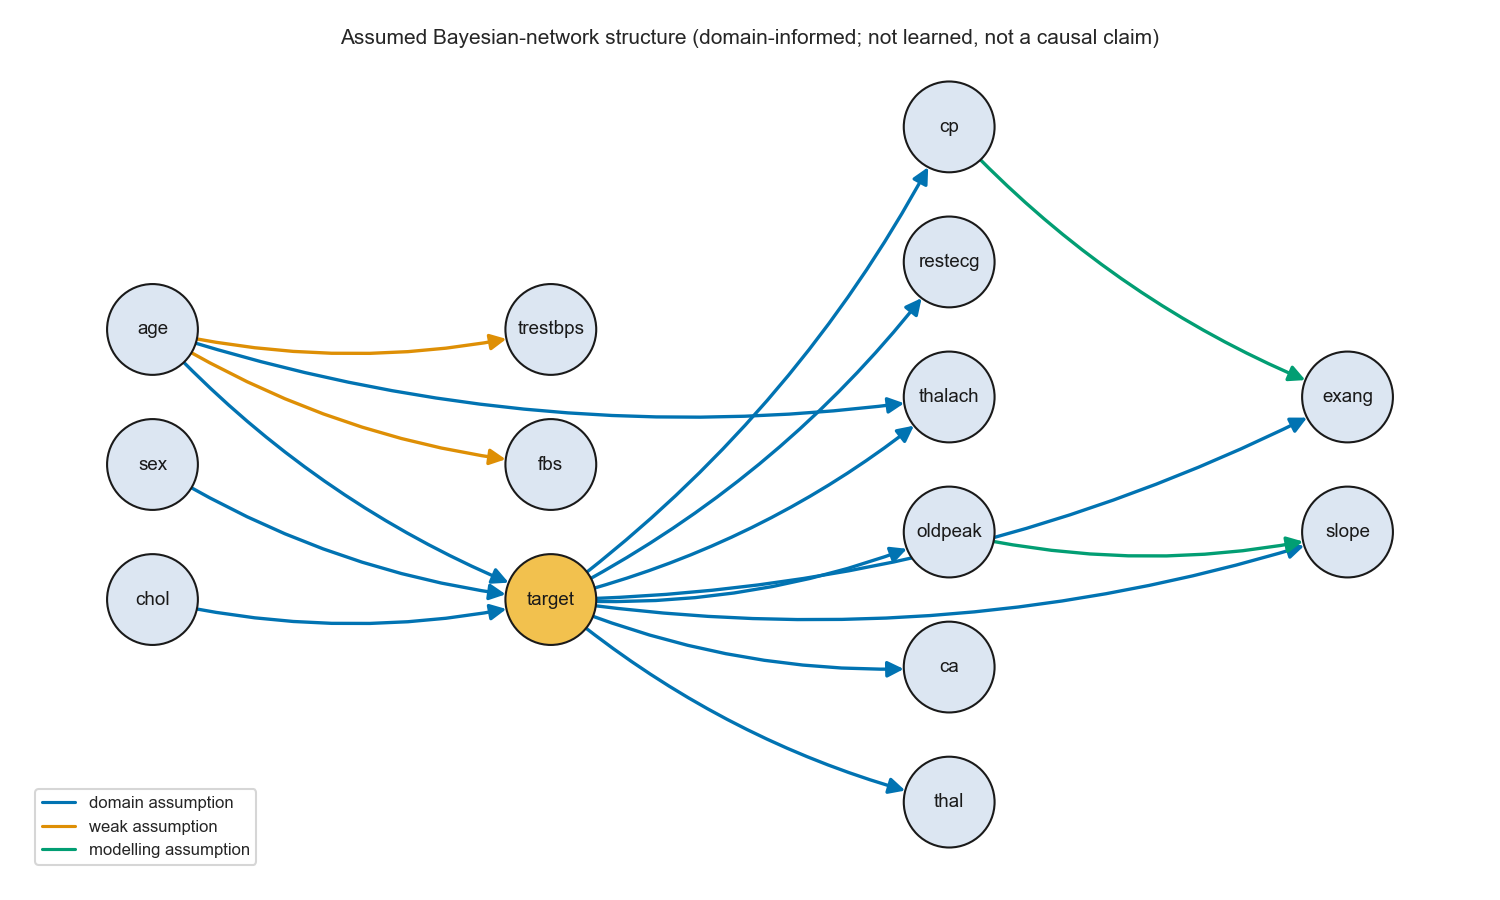
\includegraphics[width=0.78\textwidth]{bn_structure.png}
\caption{Assumed Bayesian-network structure. Colours indicate the kind of assumption. The structure is domain-informed, not learned, and not a causal claim.}
\label{fig:bn}
\end{figure*}

%--------------------------------------------------------------------
\section{MLP Architecture and Training}
The network has 20 inputs, hidden layers of 16 and 8 ReLU units each followed by dropout, and a single output logit: \nParamsMLP\ trainable parameters for about 240 training rows per fold. This is deliberately small. It is trained with the binary cross-entropy of Section~\ref{sec:theory}, Adam (learning rate $10^{-3}$), mini-batches of 32 and at most 300 epochs, implemented in PyTorch \cite{paszke2019}.

\textbf{Early stopping.} A stratified 20\% of the \emph{training fold} is held out; training stops when its loss has not improved by $10^{-4}$ for 20 epochs, and the best-epoch weights are restored. The outer validation fold is never used. Because preprocessing is fitted on the whole training fold, the inner hold-out rows influenced the scaling statistics (not the weights), a minor inner-loop leak that does not touch the outer fold.

\textbf{Fixed and tuned settings.} Hidden sizes, learning rate, batch size and the stopping rule were fixed a priori. Weight decay $\in\{10^{-3},10^{-2}\}$ and dropout $\in\{0.3,0.5\}$ were tuned in the inner loop. Fig.~\ref{fig:curves} shows the inner training and validation loss in the five repeat-0 outer folds.

\begin{figure}[t]
\centering
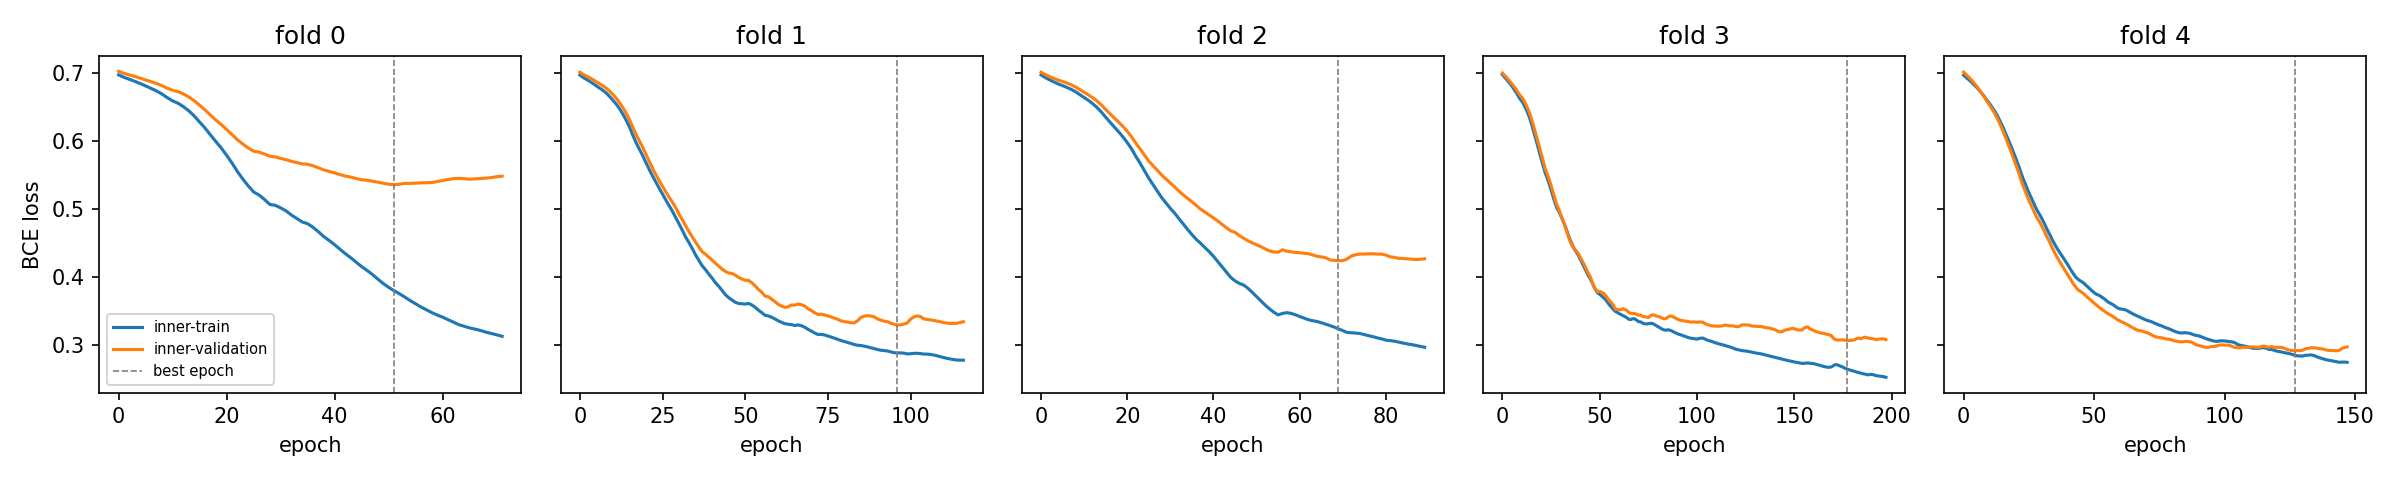
\includegraphics[width=\columnwidth]{mlp_learning_curves.png}
\caption{Learning curves (loss on the inner training split and the inner validation split) from a run with the default hyper-parameters on the five repeat-0 outer folds; the dashed line marks the best epoch.}
\label{fig:curves}
\end{figure}

%--------------------------------------------------------------------
\section{Experimental Design and Evaluation Metrics}
\textbf{Outer folds.} All models use the same stratified $5$-fold cross-validation repeated $5$ times with seed $\seed$, i.e.\ $\nOuter$ outer train/validation splits (fold hash \texttt{\foldHash}). The five repeats were chosen before any result was seen, because one 5-fold split of 303 rows is noisy. Each patient receives exactly one out-of-fold prediction per repeat per model; completeness, probability validity ($\in[0,1]$, finite, $P(0)+P(1)=1$) and identical fold membership across models are asserted by the evaluation code.

\textbf{Nested tuning.} Within each outer training fold a stratified $5$-fold inner cross-validation selects hyper-parameters by inner out-of-fold log loss: Naive Bayes $\alpha\in\{0.5,1,2\}$; BN pseudo-count $\alpha\in\{0.5,1,2\}$; MLP weight decay and dropout as above. The best setting is refitted on the whole outer training fold. Outer validation labels are used only to score predictions; an automated test confirms, for the Naive Bayes and Bayesian-network pipelines, that flipping the outer validation labels leaves every prediction and selected threshold unchanged (the MLP shares the same evaluation code but is not covered by that test) \cite{varma2006,cawley2010}.

\textbf{Threshold.} Hard-label metrics use a fixed threshold of $0.5$ chosen a priori. As a secondary analysis, a Youden threshold is selected on the \emph{inner out-of-fold predictions of the training fold only} and applied to the outer fold.

\textbf{Uncertainty.} We report mean $\pm$ standard deviation over the $\nOuter$ outer folds (about 60 patients each), pooled out-of-fold metrics per repeat, and 95\% percentile intervals from $\nBoot$ patient-level bootstrap resamples, in which model differences are paired \cite{efron1993}. The fold-level SD understates uncertainty about new patients because training sets overlap, and the bootstrap resamples patients but not the training procedure.

\textbf{Reproducibility.} Seeds (outer and inner folds, MLP initialisation and batch order, bootstrap) derive from one project seed; exact package versions are listed in \texttt{requirements-lock.txt} (Python 3.9.6, scikit-learn 1.6.1, pgmpy 0.1.26, PyTorch 2.8.0). A rebuild from a clean environment reproduced the out-of-fold predictions, selected hyper-parameters and all summary tables byte for byte.

%--------------------------------------------------------------------
\section{Results and Comparative Analysis}
Table~\ref{tab:fold} gives fold-level results at threshold $0.5$, and Table~\ref{tab:ci} the pooled out-of-fold estimates with bootstrap intervals. Figs.~\ref{fig:roc} and~\ref{fig:cm} show the curves and confusion matrices.

\begin{table*}[t]
\centering
\caption{Fold-level results over $\nOuter$ outer folds (mean $\pm$ SD), threshold 0.5.}
\label{tab:fold}
\footnotesize
\resizebox{\textwidth}{!}{\begin{tabular}{lcccccccc}
\toprule
Model & ROC AUC & PR AUC & Sens. & Spec. & Prec. & F1 & Brier & Log loss \\
\midrule
Bayesian Network & 0.912 $\pm$ 0.036 & 0.911 $\pm$ 0.037 & 0.787 $\pm$ 0.083 & 0.848 $\pm$ 0.065 & 0.818 $\pm$ 0.066 & 0.799 $\pm$ 0.054 & 0.127 $\pm$ 0.030 & 0.417 $\pm$ 0.106 \\
Naive Bayes & 0.907 $\pm$ 0.033 & 0.907 $\pm$ 0.035 & 0.803 $\pm$ 0.090 & 0.850 $\pm$ 0.068 & 0.825 $\pm$ 0.072 & 0.810 $\pm$ 0.056 & 0.134 $\pm$ 0.031 & 0.465 $\pm$ 0.109 \\
MLP & 0.907 $\pm$ 0.037 & 0.905 $\pm$ 0.040 & 0.803 $\pm$ 0.080 & 0.865 $\pm$ 0.059 & 0.837 $\pm$ 0.067 & 0.817 $\pm$ 0.059 & 0.121 $\pm$ 0.025 & 0.391 $\pm$ 0.064 \\
\bottomrule
\end{tabular}
}
\end{table*}

\begin{table}[t]
\centering
\caption{Pooled out-of-fold estimates (mean over 5 repeats) with 95\% patient-level bootstrap intervals.}
\label{tab:ci}
\scriptsize
\resizebox{\columnwidth}{!}{\begin{tabular}{lccc}
\toprule
Model & ROC AUC & PR AUC & Brier \\
\midrule
Bayesian Network & 0.909 [0.873, 0.939] & 0.905 [0.860, 0.939] & 0.127 [0.099, 0.157] \\
Naive Bayes & 0.904 [0.869, 0.935] & 0.900 [0.853, 0.936] & 0.134 [0.105, 0.166] \\
MLP & 0.903 [0.868, 0.936] & 0.895 [0.851, 0.933] & 0.121 [0.099, 0.144] \\
\bottomrule
\end{tabular}
}
\end{table}

\begin{figure*}[t]
\centering
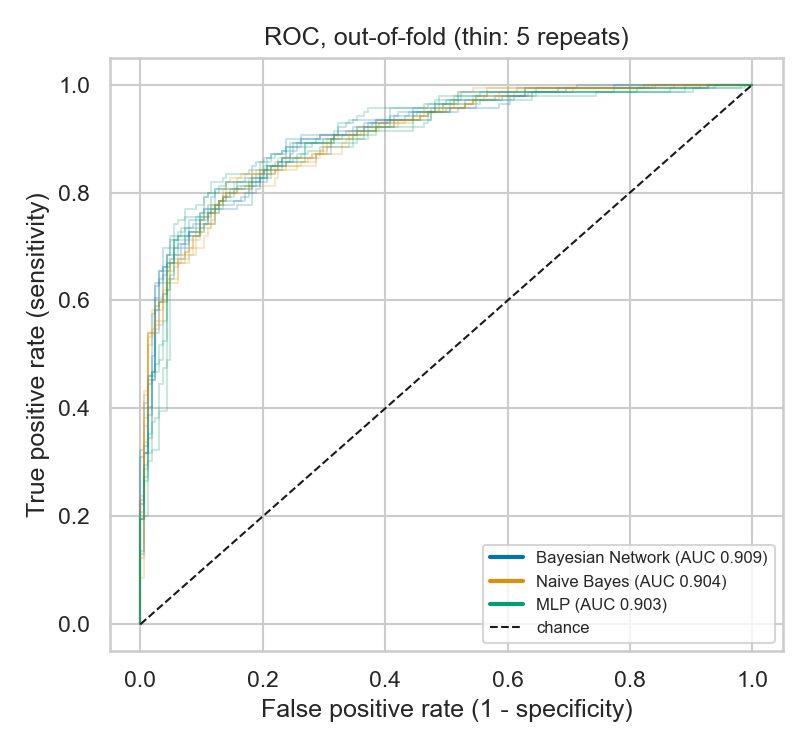
\includegraphics[width=0.36\textwidth]{roc_curves.png}\hspace{1em}
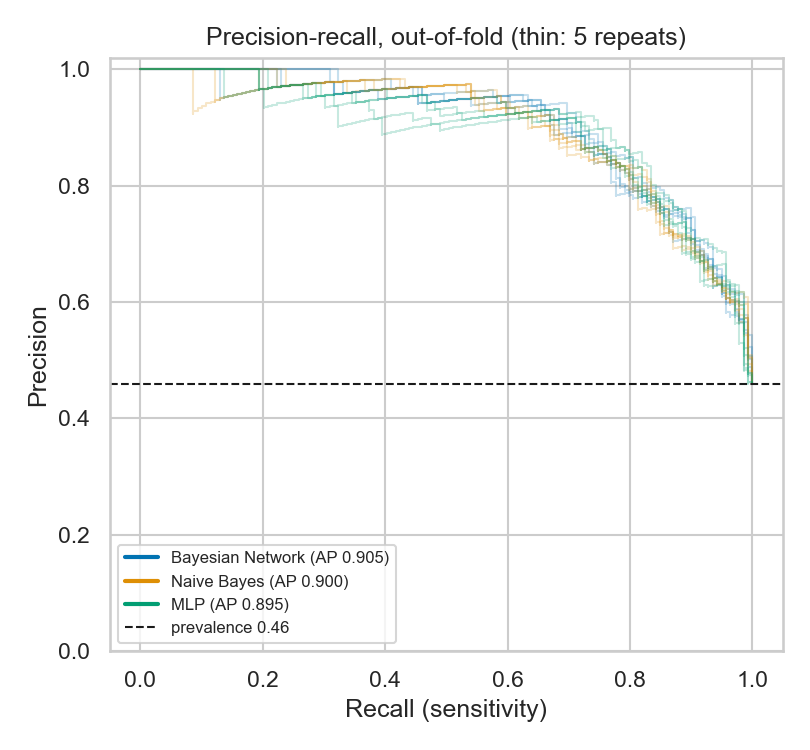
\includegraphics[width=0.36\textwidth]{pr_curves.png}
\caption{Out-of-fold ROC and precision--recall curves (thin lines: five repeats). The dashed PR line is the prevalence ($\posPct\%$).}
\label{fig:roc}
\end{figure*}

\begin{figure}[t]
\centering
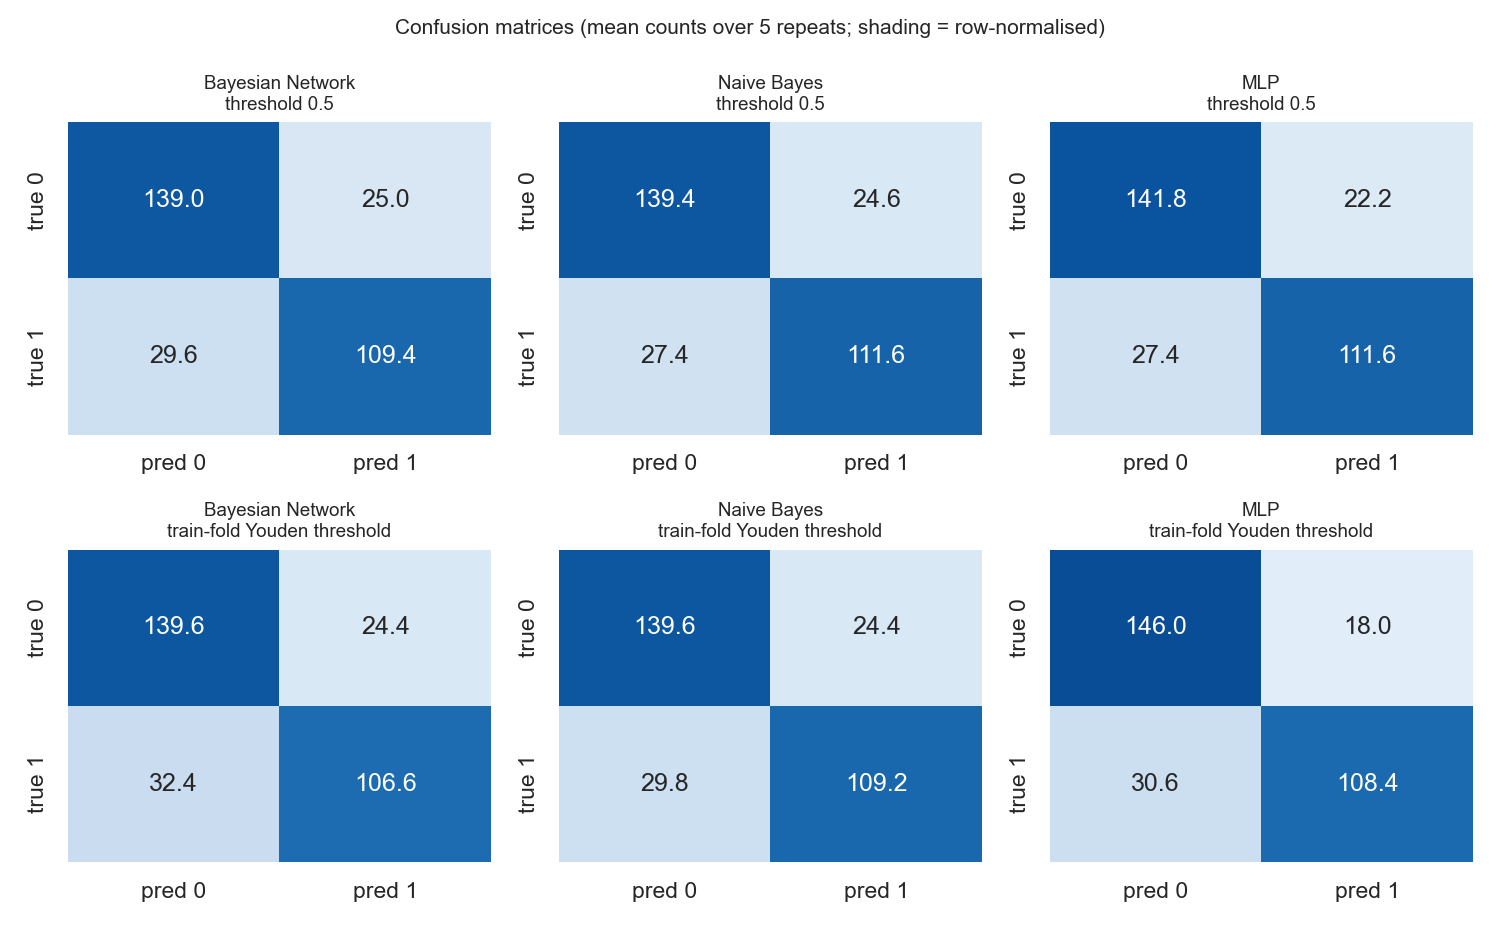
\includegraphics[width=\columnwidth]{confusion_matrices.png}
\caption{Confusion matrices (mean counts over five repeats) at threshold 0.5 (top) and the training-fold Youden threshold (bottom).}
\label{fig:cm}
\end{figure}

\textbf{Discrimination.} All three models reach ROC AUC and PR AUC of about 0.90--0.91. The Bayesian network has the nominally highest values, but the paired bootstrap differences are small and all include zero: BN$-$MLP ROC AUC $\DiffBNMLProcaucEst$ [\DiffBNMLProcaucLo, \DiffBNMLProcaucHi], BN$-$NB $\DiffBNNBrocaucEst$ [\DiffBNNBrocaucLo, \DiffBNNBrocaucHi], NB$-$MLP $\DiffNBMLProcaucEst$ [\DiffNBMLProcaucLo, \DiffNBMLProcaucHi] (Table~\ref{tab:paired}). We therefore have no evidence that one model ranks patients better. The MLP, with \nParamsMLP\ parameters, did not outperform the simpler models, in line with findings for tabular data \cite{shwartz2022,grinsztajn2022}.

\textbf{Hard-label performance.} At threshold $0.5$ sensitivity is about \BNsensMean--\NBsensMean\ and specificity about \BNspecMean--\MLPspecMean, with fold-level SDs of 0.06--0.09, which correspond to only about five patients per fold. On average \BNfnP\ (BN), \NBfnP\ (NB) and \MLPfnP\ (MLP) of the $\nPos$ diseased patients are missed per repeat (Table~\ref{tab:conf}); in any screening-type setting this is a substantial weakness.

\begin{table}[t]
\centering
\caption{Paired bootstrap differences (first minus second model), 95\% intervals.}
\label{tab:paired}
\scriptsize
\resizebox{\columnwidth}{!}{\begin{tabular}{llccc}
\toprule
Comparison & Metric & Difference & 95\% CI & Includes 0 \\
\midrule
BN $-$ NB & ROC AUC & +0.004 & [-0.004, +0.013] & yes \\
BN $-$ NB & PR AUC & +0.005 & [-0.004, +0.015] & yes \\
BN $-$ NB & Brier & -0.008 & [-0.017, +0.002] & yes \\
BN $-$ NB & Log loss & -0.048 & [-0.081, -0.018] & no \\
BN $-$ MLP & ROC AUC & +0.005 & [-0.012, +0.021] & yes \\
BN $-$ MLP & PR AUC & +0.010 & [-0.011, +0.032] & yes \\
BN $-$ MLP & Brier & +0.005 & [-0.008, +0.019] & yes \\
BN $-$ MLP & Log loss & +0.025 & [-0.027, +0.080] & yes \\
NB $-$ MLP & ROC AUC & +0.001 & [-0.014, +0.016] & yes \\
NB $-$ MLP & PR AUC & +0.005 & [-0.016, +0.028] & yes \\
NB $-$ MLP & Brier & +0.013 & [-0.002, +0.029] & yes \\
NB $-$ MLP & Log loss & +0.073 & [+0.007, +0.145] & no \\
\bottomrule
\end{tabular}
}
\end{table}

\begin{table}[t]
\centering
\caption{Mean confusion counts per repeat (303 patients).}
\label{tab:conf}
\footnotesize
\begin{tabular}{llcccc}
\toprule
Model & Threshold & TN & FP & FN & TP \\
\midrule
Bayesian Network & 0.5 & 139.0 & 25.0 & 29.6 & 109.4 \\
Bayesian Network & Youden & 139.6 & 24.4 & 32.4 & 106.6 \\
Naive Bayes & 0.5 & 139.4 & 24.6 & 27.4 & 111.6 \\
Naive Bayes & Youden & 139.6 & 24.4 & 29.8 & 109.2 \\
MLP & 0.5 & 141.8 & 22.2 & 27.4 & 111.6 \\
MLP & Youden & 146.0 & 18.0 & 30.6 & 108.4 \\
\bottomrule
\end{tabular}

\end{table}

\textbf{Threshold selection.} The Youden threshold selected on training data (Table~\ref{tab:thr}) did not raise sensitivity for any model; it traded sensitivity for specificity. The selected thresholds averaged \BNYoudenMean\ (BN), \NBYoudenMean\ (NB) and \MLPYoudenMean\ (MLP) but ranged from \BNYoudenMin\ to \NBYoudenMax\ across folds, i.e.\ they are unstable at this sample size, so $0.5$ is retained as the reported threshold.

\begin{table}[t]
\centering
\caption{Sensitivity and specificity (fold-level, mean $\pm$ SD) at the fixed and the training-fold Youden threshold.}
\label{tab:thr}
\scriptsize
\begin{tabular}{llcc}
\toprule
Model & Threshold & Sensitivity & Specificity \\
\midrule
Bayesian Network & 0.5 & 0.787 $\pm$ 0.083 & 0.848 $\pm$ 0.065 \\
Bayesian Network & Youden & 0.767 $\pm$ 0.109 & 0.851 $\pm$ 0.090 \\
Naive Bayes & 0.5 & 0.803 $\pm$ 0.090 & 0.850 $\pm$ 0.068 \\
Naive Bayes & Youden & 0.786 $\pm$ 0.087 & 0.851 $\pm$ 0.075 \\
MLP & 0.5 & 0.803 $\pm$ 0.080 & 0.865 $\pm$ 0.059 \\
MLP & Youden & 0.780 $\pm$ 0.083 & 0.890 $\pm$ 0.064 \\
\bottomrule
\end{tabular}

\end{table}

\textbf{Selected hyper-parameters.} The BN pseudo-count and the Naive Bayes $\alpha$ selected the largest grid value ($2.0$) in \BNalphaTop\ and \NBalphaTop\ of $\nOuter$ folds, respectively, so the grid was too narrow at its upper end. The MLP chose weight decay $10^{-2}$ in \WDhigh\ folds and $10^{-3}$ in \WDlow, and dropout $0.5$ in \DOhigh\ folds and $0.3$ in \DOlow.

\textbf{Class imbalance.} With $\posPct\%$ positives, imbalance is mild, PR AUC tracks ROC AUC, and no resampling or class weights were used.

%--------------------------------------------------------------------
\section{Interpretation and Probability Calibration}
\label{sec:cal}
\textbf{Calibration.} Probability quality differs more than ranking (Table~\ref{tab:cal}, Fig.~\ref{fig:cal}). The MLP has the lowest Brier score (\MLPbrierEst\ vs.\ \BNbrierEst\ and \NBbrierEst), log loss and ECE, and a calibration slope of \MLPcalslopePMean, close to the ideal $1$. The Bayesian network (\BNcalslopePMean) and Naive Bayes (\NBcalslopePMean) are over-confident: \BNHiShare\% and \NBHiShare\% of their out-of-fold predictions are $\ge0.9$ (MLP: \MLPHiShare\%), yet the observed positive rate in that group is \BNHiObs\ and \NBHiObs\ against mean predictions of \BNHiPred\ and \NBHiPred. Among predictions $\le0.1$ the observed positive rate is \BNLoObs\ (BN) and \NBLoObs\ (NB) against mean predictions of \BNLoPred\ and \NBLoPred. Naive Bayes is worst, consistent with its violated independence assumption; the BN's few extra edges only partly repair this. In the paired bootstrap, the log-loss difference excludes zero for NB$-$MLP ($\DiffNBMLPloglossEst$ [\DiffNBMLPloglossLo, \DiffNBMLPloglossHi]) and BN$-$NB ($\DiffBNNBloglossEst$ [\DiffBNNBloglossLo, \DiffBNNBloglossHi]) but not for BN$-$MLP; no Brier-score difference excludes zero. Because many metrics and comparisons were examined without multiplicity correction, the calibration finding is suggestive rather than confirmatory. The over-confidence of BN and NB may also be partly due to the truncated smoothing grid.

\begin{table}[t]
\centering
\caption{Calibration (pooled out-of-fold, per repeat; mean $\pm$ SD over 5 repeats). Ideal slope 1, intercept 0.}
\label{tab:cal}
\footnotesize
\begin{tabular}{lccc}
\toprule
Model & ECE & Cal.\ slope & Cal.\ intercept \\
\midrule
Bayesian Network & 0.082 $\pm$ 0.003 & 0.62 $\pm$ 0.01 & -0.06 $\pm$ 0.03 \\
Naive Bayes & 0.101 $\pm$ 0.010 & 0.51 $\pm$ 0.00 & -0.05 $\pm$ 0.02 \\
MLP & 0.059 $\pm$ 0.009 & 1.10 $\pm$ 0.05 & 0.09 $\pm$ 0.10 \\
\bottomrule
\end{tabular}

\end{table}

\begin{figure}[t]
\centering
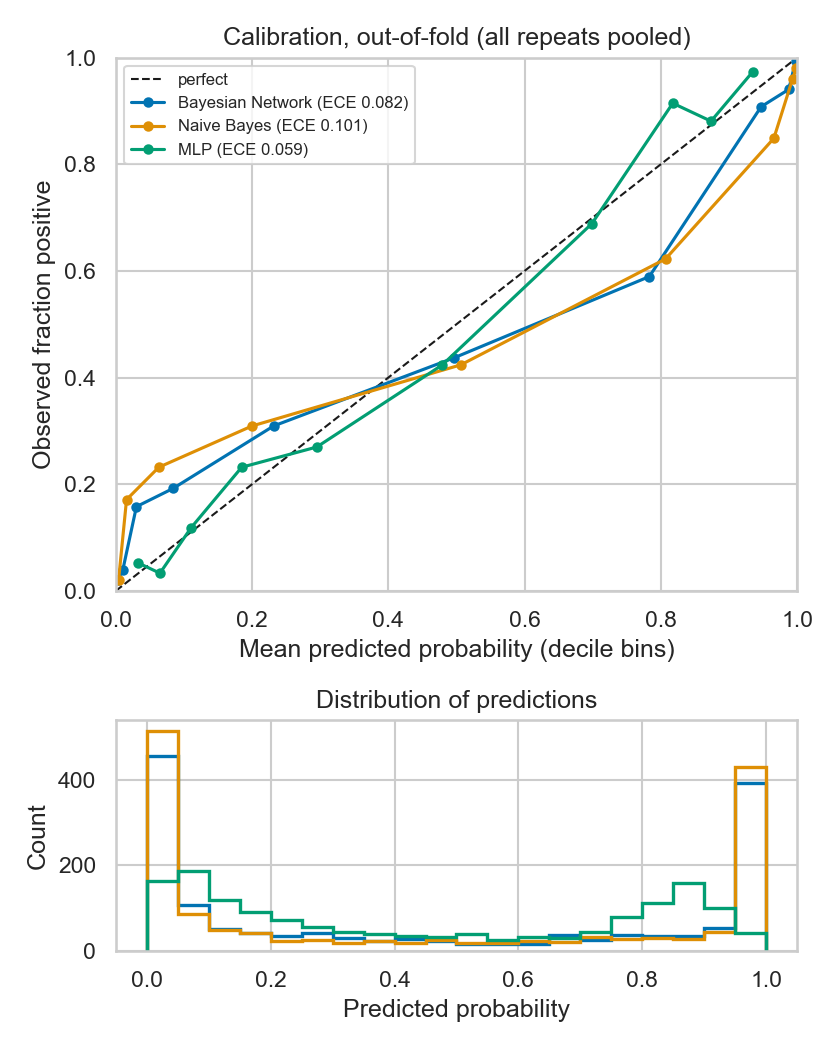
\includegraphics[width=0.88\columnwidth]{calibration_curves.png}
\caption{Reliability curves (decile bins, all repeats pooled) and prediction histograms. The Bayesian network and Naive Bayes concentrate predictions near 0 and 1.}
\label{fig:cal}
\end{figure}

\textbf{Feature attribution for the MLP.} For the five repeat-0 outer folds, each MLP was refitted with its selected hyper-parameters (reproducing the saved out-of-fold predictions to $10^{-16}$), and the held-out rows were explained with SHAP \cite{lundberg2017} (Kernel explainer on the 13 raw predictors) and by permutation importance (drop in ROC AUC). Table~\ref{tab:attr} and Fig.~\ref{fig:attr} show that both methods rank \texttt{ca}, \texttt{cp} and \texttt{thal} highest, followed by \texttt{oldpeak}; \texttt{fbs}, \texttt{chol} and \texttt{age} contribute little. This describes \emph{what the fitted model uses}, not what causes disease: correlated predictors share or hide credit (a low rank for \texttt{age} does not mean age is irrelevant, since \texttt{ca} and \texttt{thalach} partly encode it), the folds contain only about 60 rows so several permutation intervals span zero, the Kernel explainer is a sampling approximation, and the three leading features come from invasive or specialist tests. Post-hoc attributions should not be mistaken for explanations of the underlying phenomenon \cite{rudin2019}.

\begin{table}[t]
\centering
\caption{MLP feature attribution on held-out rows (repeat-0 outer folds).}
\label{tab:attr}
\scriptsize
\begin{tabular}{lcc}
\toprule
Feature & mean $|$SHAP$|$ & AUC drop (permutation) \\
\midrule
\texttt{ca} & 0.104 & 0.054 $\pm$ 0.017 \\
\texttt{cp} & 0.089 & 0.035 $\pm$ 0.014 \\
\texttt{thal} & 0.085 & 0.028 $\pm$ 0.013 \\
\texttt{oldpeak} & 0.055 & 0.010 $\pm$ 0.014 \\
\texttt{slope} & 0.044 & 0.002 $\pm$ 0.004 \\
\texttt{trestbps} & 0.039 & 0.005 $\pm$ 0.013 \\
\texttt{thalach} & 0.038 & 0.006 $\pm$ 0.003 \\
\texttt{sex} & 0.024 & 0.006 $\pm$ 0.008 \\
\texttt{exang} & 0.024 & 0.004 $\pm$ 0.001 \\
\texttt{restecg} & 0.022 & 0.001 $\pm$ 0.003 \\
\texttt{chol} & 0.011 & -0.002 $\pm$ 0.002 \\
\texttt{age} & 0.005 & 0.001 $\pm$ 0.003 \\
\texttt{fbs} & 0.002 & -0.002 $\pm$ 0.003 \\
\bottomrule
\end{tabular}

\end{table}

\begin{figure*}[t]
\centering
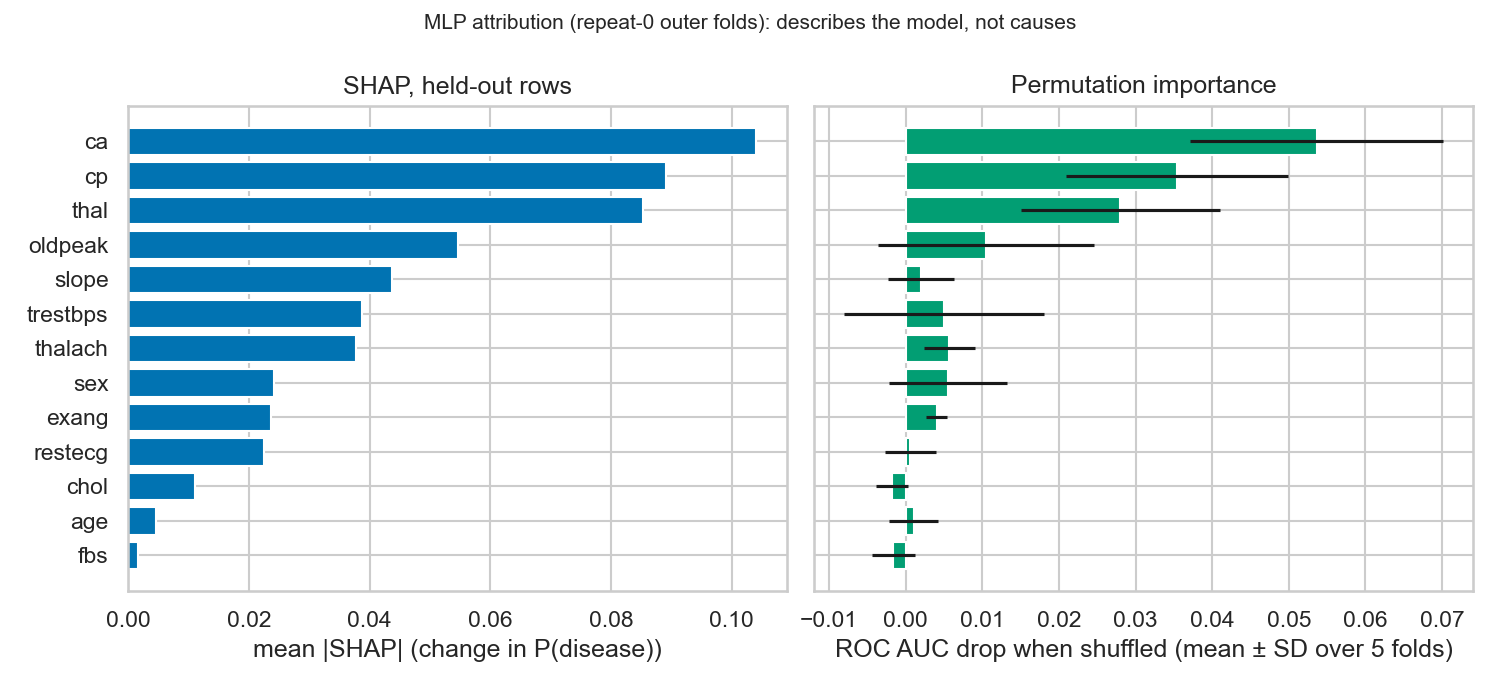
\includegraphics[width=0.75\textwidth]{mlp_attribution_bars.png}
\caption{SHAP and permutation importance for the MLP. These describe the fitted model, not causal effects.}
\label{fig:attr}
\end{figure*}

%--------------------------------------------------------------------
\section{Limitations and Ethical Considerations}
\textbf{Data.} 303 patients from one centre and period; no external validation. Internal cross-validation cannot support clinical validity or generalisability. All patients were assessed for coronary disease, so prevalence ($\posPct\%$) is not a population rate, and referral bias is likely. Predictors include exercise-test, fluoroscopy and perfusion-imaging results, so the models do not apply to first-contact triage. The binary target pools four severity levels. Sparse categories make table estimates unstable. The sample has more men (206) than women (97), limiting subgroup conclusions; no fairness analysis was performed.

\textbf{Methods.} Missing values are filled with the training mode. Differences between models lie within the noise, and 36 bootstrap intervals were inspected without correction for multiplicity. The BN structure is an a-priori assumption (one edge was suggested by exploratory analysis of the full sample). The tuning grid for BN and Naive Bayes was truncated at its upper end in every fold; we did not widen it after seeing outer-fold results, so as to avoid outcome-informed changes, and doing so would be a new pre-declared experiment. MLP early-stopping rows influenced scaling statistics (not weights). Attribution results are not causal.

\textbf{Ethics.} The data are a publicly released research dataset under CC BY 4.0 that, according to its documentation, has had patient names and social-security numbers removed, and the data owners request that publications acknowledge the investigators responsible for the data \cite{uciheart,detrano1989}. A model like this must not be used for patient care: it has not been validated prospectively or externally, is trained on historical data from one population, and would be subject to automation bias if shown to clinicians. Over-confident probabilities (Section~\ref{sec:cal}) would be especially harmful in a decision-support setting. Any clinical application would require external validation, calibration monitoring, subgroup analysis and regulatory review, and reporting guidance such as TRIPOD \cite{collins2015}.

%--------------------------------------------------------------------
\section{Conclusion and Future Work}
Under an identical, leakage-safe nested cross-validation protocol, a domain-informed Bayesian network, Naive Bayes and a small MLP achieved indistinguishable discrimination on the Cleveland data (ROC AUC about 0.90--0.91; sensitivity about 0.79--0.80 and specificity about 0.85--0.87 at threshold 0.5). The principal difference is probability quality: the MLP's probabilities were better calibrated, while the Bayesian network and Naive Bayes were over-confident. Because of the small single-centre sample, wide uncertainty and the exploratory nature of the calibration comparison, we draw no claim of general superiority and no clinical claim. A Streamlit application accompanies the code so that readers can explore the data, the saved evaluation results and the three models on a hypothetical profile; it displays the saved results without re-estimating them, refits the models on all 303 rows only for the demonstration, and carries the same disclaimer as this paper.

Future work should (i) pre-declare and run wider smoothing grids and post-hoc recalibration (e.g.\ Platt scaling or isotonic regression fitted in the inner loop) for BN and Naive Bayes, (ii) learn or test the BN structure with structure-learning methods and compare it with the expert structure, (iii) handle missing values by multiple imputation or exact marginalisation, (iv) add external validation on the other hospital subsets of the same archive and on independent cohorts, (v) report subgroup performance, and (vi) repeat the study with additional tabular baselines.

\bibliographystyle{IEEEtran}
\bibliography{references}

\end{document}
